\begin{enumerate}
\setcounter{figure}{0}
\renewcommand{\thefigure}{\theenumi.\arabic{figure}}

\item In Fig. 	\ref{fig:3.5.4_quadrilateral1}
\begin{align}
 \vec{P} - \vec{S} &= 
 \vec{Q} - \vec{R} = \myvec{2\\-2}
\\
\vec {R} - \vec {S} &=
 \vec {Q} - \vec {P} = \myvec{2\\2}
\end{align}
%
Hence $PQRS$ is a $\parallel$gm $\because$  opposite sides are parallel. Also, 
\begin{align}
\norm{ \vec{P} - \vec{S}} &= 
\norm{ \vec{Q} - \vec{R}} 
\\
=\norm{\vec {R} - \vec {S}} &=
\norm{ \vec {Q} - \vec {P}} = 2\sqrt{2}
\end{align}
%
$\because$ all sides are equal, the $\parallel$gm is a rhombus.

\begin{figure}[!ht]
	\centering
	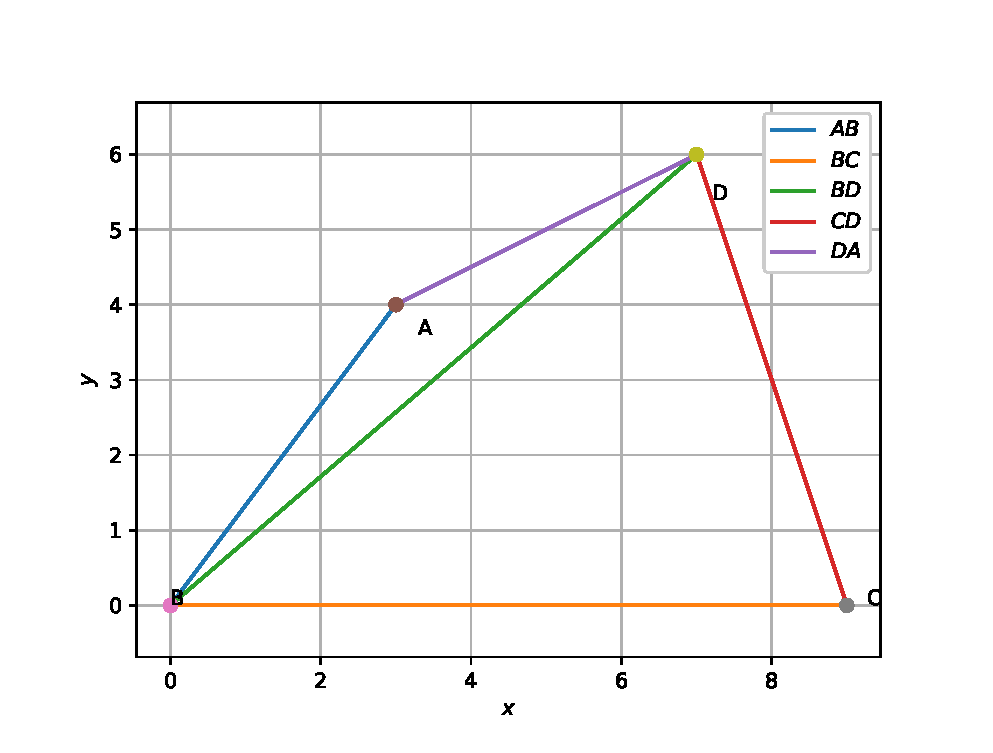
\includegraphics[width=\columnwidth]{./solutions/4/figures/line/quads/quad1.eps}
	\caption{quadrilateral1 }
	\label{fig:3.5.4_quadrilateral1}
\end{figure}
\begin{lstlisting}
solutions/4/codes/line/quad/quad1.py
\end{lstlisting}

\item In Fig. 	\ref{fig:3.5.4_quadrilateral2}

\begin{align}
\vec{Q} - \vec{P} &= \myvec{6\\-4}
\\
\vec{R} - \vec{P} &= \myvec{3\\-2}
\\
\vec{Q} - \vec{R} &= \myvec{3\\-2}
\\
\left(\vec{Q} - \vec{P}\right) &= \left(\vec{R} - \vec{P}\right) + \left(\vec{Q} - \vec{R}\right) = \myvec{6\\-4}
\end{align}
Hence,  $\vec P,\vec Q$ and $\vec R$ lie on a straight line, so $PQRS$ is not  a quadrilateral.

\begin{figure}[!ht]
	\centering
	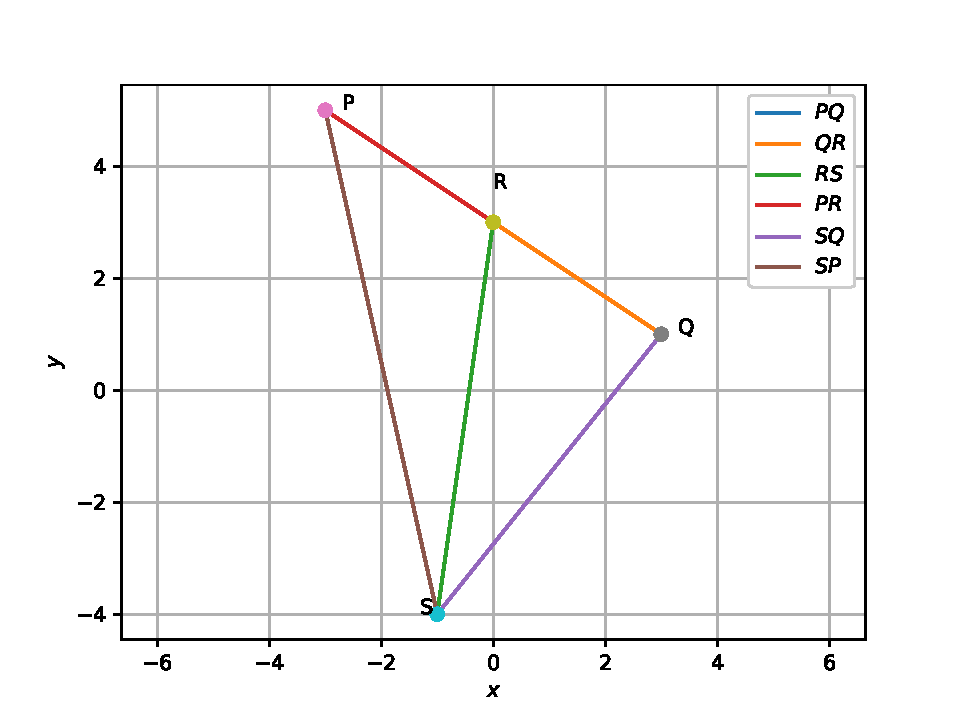
\includegraphics[width=\columnwidth]{./solutions/4/figures/line/quads/quad2.eps}
	\caption{quadrilateral2 }
	\label{fig:3.5.4_quadrilateral2}
\end{figure}
\begin{lstlisting}
/solutions/4/codes/line/quad/quad2.py
\end{lstlisting}

\item See Fig. 	\ref{fig:3.5.4_quadrilateral3}.

\begin{align}
\because \left(\vec{Q} - \vec{P}\right) &= \left(\vec{R} - \vec{S}\right) = \myvec{3\\1}
\\
\left(\vec{P} - \vec{S}\right) &= \left(\vec{Q} - \vec{R}\right) = \myvec{3\\3},
\end{align}
$PQRS$ is a parallelogram.  Also, 
%
\begin{align}
\norm{\vec{Q} - \vec{P}} \ne \norm{\vec{P} - \vec{S}}
\end{align}
Hence, $PQRS$ is neither a rhombus nor a square.
\begin{align}
\because \left(\vec{Q} - \vec{P}\right)^T \left(\vec{Q} - \vec{R}\right) = \myvec{3 & 1}\myvec{3\\3} \ne 0,
\end{align}
$PQRS$ is not a rectangle. The following code generates Fig. 	\ref{fig:3.5.4_quadrilateral3}.
	\begin{lstlisting}
	solutions/4/codes/line/quad/quad3.py
	\end{lstlisting}

\begin{figure}[!ht]
	\centering
	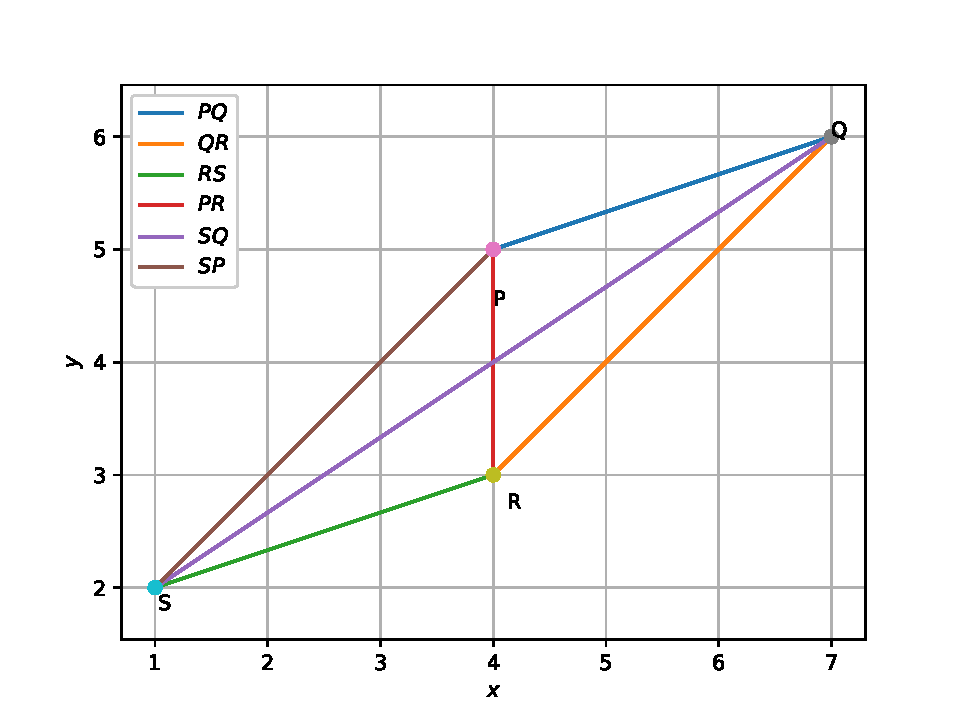
\includegraphics[width=\columnwidth]{./solutions/4/figures/line/quads/quad3.eps}
	\caption{}
	\label{fig:3.5.4_quadrilateral3}
\end{figure}
\renewcommand{\thefigure}{\theenumi}

\end{enumerate}
